\scanpage{116}
\mspage{115}


\uline{Chapter} 1\qquad Generalities on $\unsure{\otimes|\Omega}$-categories.

\margin{\handwritten{\deleted{\unsure{categories} \illegible{1} \unsure{examples}.}\par
\textcircled{1} tensor product of modules\par
\textcircled{2} category with cartesian products\par
\textcircled{3} torsors under an abelian sheaf\par
\textcircled{4} families of modules \unsure{indexed} by \unsure{gr.}\par
\textcircled{5} loop space of a \fbox{topological} space}}

\uline{Paragraph}.0: $\otimes$ laws on a category: various examples ....

\uline{Paragraph}.1 \deleted{\unsure{,|I.} The data} Constraints for a $\otimes$ law .

1.1. Associativity.

1.2. Commutativity.

1.3. Units.

1.4. $\underline{\mathrm{Hom}}(X,Y),\ \underline{\mathrm{Moh}}(Y,X)$\handwritten{;} \deleted{$X^{\handwritten{\unsure{\vee}}}$} .

\inserted{\handwritten{\figure{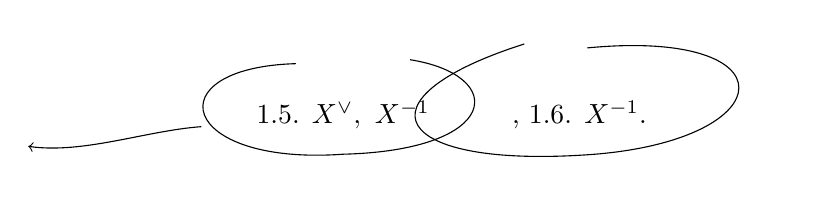
\begin{tikzpicture}[x=1cm,y=1cm]
\node at (0,0) {1.5. $X^\vee,\ X^{-1}$};
\node at (3,0) {, \deleted{\unsure{1.6.}} $X^{-1}$.};
\draw[<-] (-4,-.4) .. controls (-3.3,-.5) and (-2.5,-.2) .. (-1.8,-.15);
\draw (-.6,.65) .. controls (-2.4,.6) and (-2.1,-.65) .. (0,-.5) .. controls (2,-.45) and (2.1,.5) .. (.85,.7);
\draw (2.3,.9) .. controls (.1,.2) and (.6,-.7) .. (3.2,-.5) .. controls (5.6,-.3) and (5.7,1.1) .. (3.1,.85);
\end{tikzpicture}}}}

\inserted{\handwritten{1.6. Case of the examples of Paragraph 0}}

\uline{Paragraph}.2\qquad Compatibilities between constraints. \handwritten{\figure{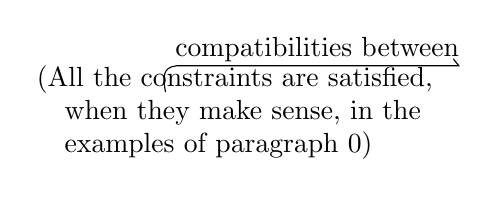
\begin{tikzpicture}[x=1em,y=1em]
\node[anchor=west] at (0,0) {(All the constraints are satisfied,};
\node[anchor=west] at (1,-1.2) {when they make sense, in the};
\node[anchor=west] at (1,-2.4) {examples of paragraph 0)};
\node[anchor=west] at (5,1.1) {\inserted{compatibilities between}};
\draw (5,-.45) .. controls (4.9,.1) and (4.9,.45) .. (5.4,.5) -- (15.6,.5) -- (15.4,.75);
\end{tikzpicture}}}

1.1. Associativity an\unsure{\rlap{r}d|\rlap{n}d} commutativity.

1.\rlap{1}2. Commutativity and unit.

1.3. Associativity and unit.

1.4. \uline{Hom}, \uline{Moh} and associativity: Cartan's formulas.

1.5. \uline{Hom} and commutativity (one then has $\underline{\mathrm{Hom}}\inserted{\handwritten{(X,Y)\figure{\begin{tikzpicture}[x=1em,y=1em,baseline]\draw (0,.9) .. controls (.2,.8) and (.5,.55) .. (.5,0) .. controls (.6,-.2) and (.85,-.25) .. (1,-.2);\end{tikzpicture}}}}\handwritten{\simeq}\underline{\mathrm{Moh}}\handwritten{(Y,X)}$\handwritten{)}.\handwritten{-\, -\, -}

\inserted{\handwritten{\deleted{(Rigid $\otimes$ laws)}}}
\figure{
\begin{tikzpicture}[x=1em,y=1em]
\draw (0,.7) .. controls (-.3,-.1) and (.5,-.4) .. (3.5,-.35) .. controls (5.5,-.3) and (6.1,-.1) .. (6.4,.45);
\draw (6.4,.7)--(6.9,-.15)--(7.15,.8);
\end{tikzpicture}}

1.6. \unsure{\uline{Hom} and unit|\deleted{\uline{Hom} and unit}} : definition of $X^{\handwritten{\vee}}$ (for a commutative law only ?).\margin{\figure{
\begin{tikzpicture}[baseline]\node at (0,.4) {\handwritten{\uline{no!}}};\draw (.4,.2) .. controls (.8,.4) and (1,.2) .. (1.2,-.2);\draw (1.1,-.1)--(1.35,.75);\end{tikzpicture}}}

1.7. \inserted{\handwritten{\figure{
\begin{tikzpicture}[x=1em,y=1em]
\node[anchor=west] at (0,0) {\uline{Rigid} $\otimes$ laws.};
\draw (-.2,-.7) .. controls (.1,-.55) and (.8,-.65) .. (3.2,-.5) -- (3.2,.25);
\draw (5.3,.3) .. controls (6.3,.2) and (8.6,-.2) .. (10.3,-1.2);
\end{tikzpicture}}}} \handwritten{(}Formalism of traces (case \deleted{\illegible{1}} of isomorphism $X^{\handwritten{\vee}}\otimes Y\handwritten{\unsure{\simeq|\xleftarrow{\sim}}}\underline{\mathrm{Hom}}(X,Y)$)\handwritten{; rank of an object.}

\inserted{\handwritten{\uline{Paragraph}.3}} \deleted{1.8.} Norm\rlap{a}l forms of composite multifunctors. \handwritten{\deleted{(after the \uuline{\unsure{following}} §)}}

\uline{Paragraph} \deleted{3}\handwritten{4}.\qquad $\otimes$-functors.

\deleted{3}\handwritten{4}.1. Theory without constraints: definition of $\otimes$-functors, composition, morphisms of $\otimes$-functors.

\deleted{3}\handwritten{4}.2. Compatibility \rlap{o}\handwritten{o}\rlap{v}\handwritten{f}\rlap{ }\handwritten{ }\rlap{a}\handwritten{a} $\otimes$-functor with constraints: associativity and commutativity\handwritten{!}

\deleted{3}\handwritten{4}.3. Compatibility with constraints: unit.

\deleted{3}\handwritten{4}.4. Compatibility with constraints: \uline{Hom}, \uline{Moh}, \handwritten{$X^\vee,X^{-1}$ ---}

\inserted{\handwritten{4.5. Quasi-invertible objects, and \deleted{\unsure{enlargement} \unsure{of} \unsure{categories}} \inserted{calculus} of fractions....}}

\uline{Paragraph}. \deleted{4}\handwritten{5}.\qquad \uline{Typical examples;}\deleted{\unsure{the}} $\otimes$-\uline{categories}\handwritten{\uline{defined by bialgebras}.}

\inserted{\handwritten{5.0. $\otimes$-Categories; additive categories, with $\otimes$ biadditive, associative commutative unital \deleted{\unsure{with}} (not necessarily\ \uline{$\unsure{\mathrm{Huy}|\mathrm{Hom}}$}).}}

\deleted{4}\handwritten{5}.1. Modules over a bialgebra.

\deleted{4}\handwritten{5}.2. Comodules over a bialgebra.

\deleted{4}\handwritten{5}.3. Duality between the two notions: first ma\rlap{j}nner (imperfect).

\deleted{4}\handwritten{5}.4. Duality between the two notions: second manner, formal (via \deleted{\unsure{noti}} notions of algebra in a $\otimes$-category ).

\inserted{\handwritten{5.5. Mixed modules (comodule + ordinary) over a bialgebra}}
